\documentclass{beamer}

\mode<presentation> 
{
    % The Beamer class comes with a number of default slide themes
    % which change the colors and layouts of slides. Below this is a list
    % of all the themes, uncomment each in turn to see what they look like.

    %\usetheme{default}
    %\usetheme{AnnArbor}
    %\usetheme{Antibes}
    %\usetheme{Bergen}
    %\usetheme{Berkeley}
    %\usetheme{Berlin}
    %\usetheme{Boadilla}
    %\usetheme{CambridgeUS}
    %\usetheme{Copenhagen}
    %\usetheme{Darmstadt}
    %\usetheme{Dresden}
    %\usetheme{Frankfurt}
    %\usetheme{Goettingen}
    %\usetheme{Hannover}
    %\usetheme{Ilmenau}
    %\usetheme{JuanLesPins}
    %\usetheme{Luebeck}
    \usetheme{Madrid}
    %\usetheme{Malmoe}
    %\usetheme{Marburg}
    %\usetheme{Montpellier}
    %\usetheme{PaloAlto}
    %\usetheme{Pittsburgh}
    %\usetheme{Rochester}
    %\usetheme{Singapore}
    %\usetheme{Szeged}
    %\usetheme{Warsaw}

    % As well as themes, the Beamer class has a number of color themes
    % for any slide theme. Uncomment each of these in turn to see how it
    % changes the colors of your current slide theme.

    %\usecolortheme{albatross}
    %\usecolortheme{beaver}
    %\usecolortheme{beetle}
    %\usecolortheme{crane}
    %\usecolortheme{dolphin}
    %\usecolortheme{dove}
    %\usecolortheme{fly}
    %\usecolortheme{lily}
    %\usecolortheme{orchid}
    %\usecolortheme{rose}
    \usecolortheme{seagull}
    %\usecolortheme{seahorse}
    %\usecolortheme{whale}
    %\usecolortheme{wolverine}

%\setbeamertemplate{footline} % To remove the footer line in all slides uncomment this line
%\setbeamertemplate{footline}[page number] % To replace the footer line in all slides with a simple slide count uncomment this line

%\setbeamertemplate{navigation symbols}{} % To remove the navigation symbols from the bottom of all slides uncomment this line
}

\usepackage{graphicx} % Allows including images
\usepackage{booktabs} % Allows the use of \toprule, \midrule and \bottomrule in tables


\usepackage{beamerthemeshadow}
\usepackage{latexsym,amsbsy,amsopn,amstext,xcolor,multicol,amsmath}
\usepackage{amssymb,graphicx,wrapfig,fancybox}
\usepackage{pgf,pgfarrows,pgfnodes,pgfautomata,pgfheaps,pgfshade}
\usepackage{booktabs}
\usepackage{subfloat}
\usepackage{}
\graphicspath{{figures/}}

%----------------------------------------------------------------------------------------
%	TITLE PAGE
%----------------------------------------------------------------------------------------

%----------------------------------------------------------------------------------------
\title[Work Report]{Report on Recent Work from 2014.9 to 2014.12}

\author{Ma Xuning ~~~ Wang Zhiyong}
\institute[NKU \& \& IHEP]
{
    Nankai Univ. \&\& IHEP\\
    \medskip
    \textit{maxn@ihep.ac.cn}
}
\date{\today}

%----------------------------------------------------------------------------------------
\begin{document}
%----------------------------------------------------------------------------------------
\frame{\titlepage}
%----------------------------------------------------------------------------------------

%----------------------------------------------------------------------------------------
\section{Over View}
%----------------------------------------------------------------------------------------
\subsection{Over View}
\begin{frame}{Work Been Done}
\begin{block}{Software Learning}
\begin{itemize}
\item BOSS ( Including Analysis Code of $\rho\pi$ )
\item ROOT \&\& RooFit
\end{itemize}
\end{block}
\begin{block}{Investigation on the Subject}
\begin{itemize}
\item Study of $\psi(3686)\rightarrow \pi^0h_c, h_c\rightarrow\gamma\eta_c$ via $\eta_c$ exclusive decays (PRL \textbf{104}, 132002 (2010) )
\item Measurements of $h_c(1^P_1)$ in $\psi\prime$ Decays ( PRL \textbf{86}, 092009 (2012) )
\end{itemize}
\end{block}
\begin{block}{Research Been Done(Measure of the branching ratio of $\eta_c\rightarrow K^0_S K \pi$)}
\begin{itemize}
\item Exclusive Process of $\psi\prime\rightarrow\pi^0h_c,h_c\rightarrow\gamma\eta_c,\eta_c\rightarrow K^0_S K \pi$
\item Inclusive Process of $\psi\prime\rightarrow\pi^0h_c,h_c\rightarrow\gamma\eta_c,\eta_c\rightarrow anything$
\end{itemize}
\end{block}
\end{frame}
%----------------------------------------------------------------------------------------

%----------------------------------------------------------------------------------------
\section{Software Learning}
%----------------------------------------------------------------------------------------
\subsection{Software Learning}
\begin{frame}{Software Learning}
\begin{block}{Learn about the Software Environment}
\begin{itemize}
\item The installation of BOSS
\item The difference between different version.
\end{itemize}
\end{block}
\begin{block}{Learn about the Analysis Code of $\rho\pi$}
\begin{itemize}
\item The acquisition of the data from different sub-detectors
\item The usage of different classes of the program, such as PID, vertex fit and kinematics fit
\end{itemize}
\end{block}
\begin{block}{Learn about the ROOT and RooFit}
\begin{itemize}
\item Do histogram analysis in the self-build compiler
\item Write some ROOT/RooFit micros to analyze the data
\end{itemize}
\end{block}
\end{frame}
%----------------------------------------------------------------------------------------

%----------------------------------------------------------------------------------------
\section{Investigation on the Subject}
%----------------------------------------------------------------------------------------
\subsection{Investigation on the Subject}
\begin{frame}{Investigation on the Subject}
\begin{block}{Study of $\psi(3686)\rightarrow \pi^0h_c, h_c\rightarrow\gamma\eta_c$ via $\eta_c$ exclusive decays} 
In this paper the authors studied the $\eta_c$ exclusive decays.\\
The branching ratio of the process of $\eta_c\rightarrow K^0_S K \pi$ is measured in this paper, the value is $2.60\pm0.29\pm0.34\pm0.25\%$.\\
The error is relatively large.
\end{block}
\begin{block}{Measurements of $h_c(1^P_1)$ in $\psi\prime$ Decays} 
In this paper the authors studied $h_c$ via the inclusive process of\\
        \begin{center}
$\psi\prime\rightarrow\pi^0h_c, h_c\rightarrow\gamma\eta_c, \eta_c\rightarrow anything$.\\
        \end{center}
\end{block}
\end{frame}
%----------------------------------------------------------------------------------------

%----------------------------------------------------------------------------------------
\section{Research Been Done}
%----------------------------------------------------------------------------------------
\subsection{Main Idea of our work}
\begin{frame}
\begin{block}{The purpose of our work}
Measure the branching ratio of the process ${\eta}_c\rightarrow K_S K \pi$, reducing the relative error measured before.\\
\end{block}
\begin{block}{Methods}
\begin{itemize}
\item Fit ${\eta}_c$ with $K_S^0$, $K$ and $\pi$, requiring the reconstruction of $K_S^0$, $K$ and $\pi$(Corresponding to $N_{Obs1}$ and ${\epsilon}_1$);
\item Fit ${\eta}_c$ signal with the recoil mass of $\gamma$ and ${\pi}^0$, requiring the reconstruction of ${\pi}^0$ and ${\gamma}_{\rm E1}$(Corresponding to $N_{Obs2}$ and ${\epsilon}_2$);
\item The branching fraction will be acquired as the ratio of the two ${\eta}_c$ signal as
\begin{center}
\shadowbox{$Br({\eta}_c\rightarrow K_S^0 K \pi)=(\frac{N_{Obs1}}{N_{Obs2}}\cdot \frac{{\epsilon}_2}{{\epsilon}_1} \cdot \frac{1}{Br(K_S^0 \rightarrow {\pi}^+ {\pi}^-)})^{\frac{1}{2}}$}
\end{center}
\end{itemize}
\end{block}
\end{frame}

%----------------------------------------------------------------------------------------
\subsection{Exclusive Process}
\begin{frame}{Preliminary Selection}
\begin{block}{Selection of $\gamma$ and ${\pi}^0$}
\begin{itemize}
\item $E_{\gamma}>25 MeV$,$|\cos\theta|<0.8$ ( barrel region )
\item $E_{\gamma}>50 MeV$,$0.86<|\cos\theta|<0.92$ ( end-cap region )
%\item $450MeV < E({\gamma}_{{\rm E1}}) < 550MeV$
\item $|M_{\gamma \gamma}-m_{{\pi}^0}| < 15 MeV/c^2$ (With 1C)
\end{itemize}
\end{block}
\begin{block}{Selection of charged tracks}
\begin{itemize}
\item $ | \cos\theta |<0.93$
\item $|R_{z}|<10cm$,$R_{xy}<1cm$
\item $ |M_{\pi \pi} - m_{K_S^0} | < 20 MeV/c^2$ 
\end{itemize}
\end{block}
\shadowbox{We accept the ones with the minimum${\chi}^2={\chi}_{4C}^2+{\chi}_{1C}^2+{\chi}_{pid}^2+{\chi}_{vertex}^2$.}
\end{frame}
%----------------------------------------------------------------------------------------
\begin{frame}{Optimized Selection}
Using ROOT scripts, we got the Optimized Selection as below:
\begin{itemize}
\item $0<\chi_{4C}^2<25$;
\item $0.125<m_{\pi^0}<0.138$;
\item $0.45<E(\gamma_{E1})<0.53$;
\item $|m_{recoil}(\pi^0 \pi^0)-M_{J/\psi}|<0.033$;
\item $|m_{recoil}(\gamma)-M_{\chi_{c0}}|<0$;
\item $|m_{recoil}(\gamma)-M_{\chi_{c1}}|<0.004$;
\item $|m_{recoil}(\gamma)-M_{\chi_{c2}}|<0.002$;
\item $|m_{recoil}(\pi^+ \pi^-)-M_{J/\psi}|<0.004$.
\end{itemize}
\end{frame}
%----------------------------------------------------------------------------------------
\begin{frame}{Preliminary Results}
\begin{columns}
\begin{column}{0.5\textwidth}
\begin{center}
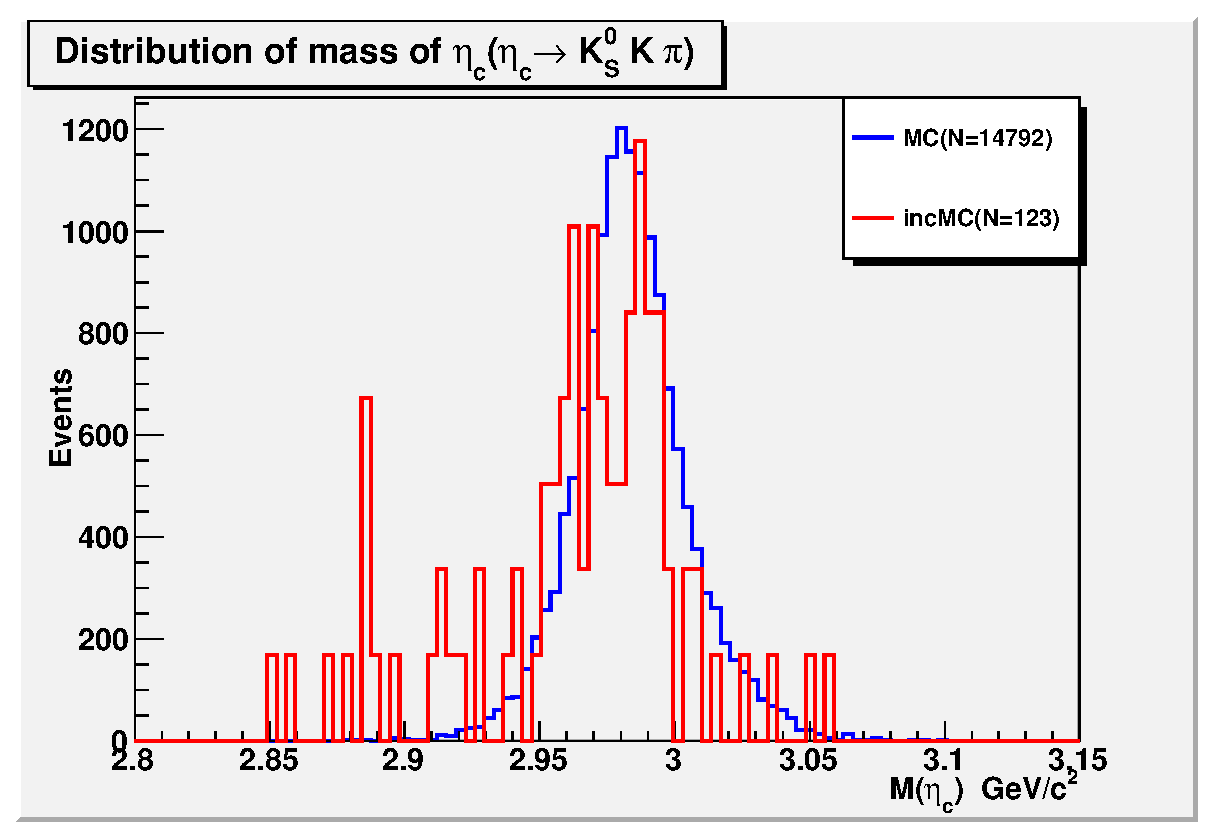
\includegraphics[width=1\textwidth,angle=0]{figures/Pi0hc_invariant_mass_of_etac.eps}\\
Mass distribution of $\eta_c$
\end{center}
\end{column}
\begin{column}{0.5\textwidth}
\begin{center}
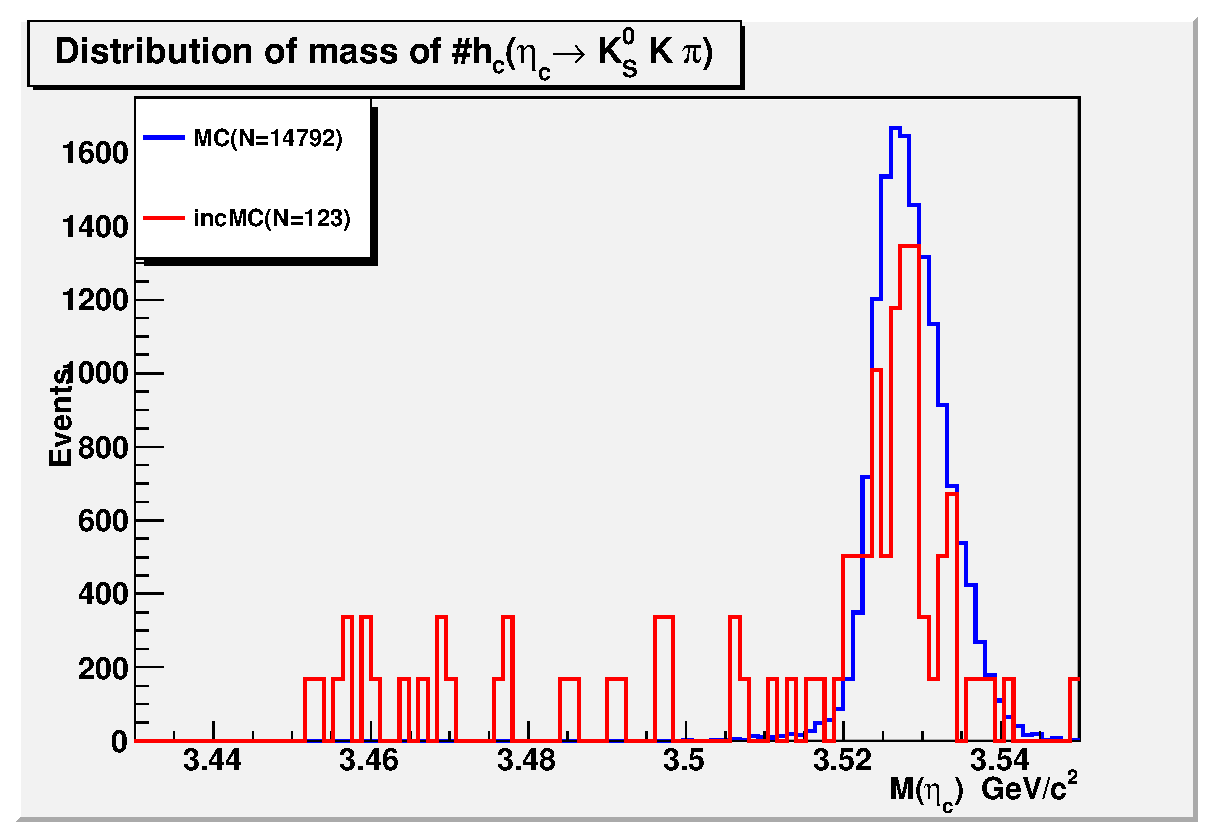
\includegraphics[width=1\textwidth,angle=0]{figures/Pi0hc_invariant_mass_of_hc.eps}\\
Mass distribution of $h_c$
\end{center}
\end{column}
\end{columns}
\end{frame}
%----------------------------------------------------------------------------------------
\begin{frame}{Topology analysis}
\vskip -1.7cm
\includegraphics[width=0.8\textwidth, angle=270]{figures/notice.eps}
\end{frame}

%----------------------------------------------------------------------------------------

%----------------------------------------------------------------------------------------
\subsection{Inclusive Process}
%----------------------------------------------------------------------------------------
\begin{frame}{Preliminary Event Selection}
\begin{block}{Selection of $\gamma_{E1}$ and $\pi^0$ candidates}
\begin{itemize}
\item $E_{\gamma}>25 MeV$,$|\cos\theta|<0.8$ ( barrel region )
\item $E_{\gamma}>50 MeV$,$0.86<|\cos\theta|<0.92$ ( end-cap region )
\item $465MeV < E({\gamma}_{{\rm E1}}) < 535MeV$
\item $120<M_{\gamma \gamma}<145 MeV/c^2$ ( With 1C )
\item photons used in $\gamma_{E1}$ candidates cannot form $\pi^0$ with another good photon
\item We keep the $\pi^0$ candidates with the minimum 1-C fit $\chi^2$ even if the daughter photons can be used in more than one $\pi^0$ candidates
\item We exclude the events with more than one $\pi^0$ in the $3.517-3.535GeV/c^2$ recoil-mass region.
\end{itemize}
\end{block}
\end{frame}
%----------------------------------------------------------------------------------------
\begin{frame}{Optimized Event Selection}
Using ROOT scripts, we got the Optimized Selection as below:
\begin{itemize}
\item $E(deposition)<0.6GeV$;
\item $|m_{recoil}(\pi^0 \pi^0)-M_{J/\psi}|<0.02$;
\item $|m_{recoil}(\gamma)-M_{\chi_{c0}}|<0.004$;
\item $|m_{recoil}(\gamma)-M_{\chi_{c1}}|<0.004$;
\item $|m_{recoil}(\gamma)-M_{\chi_{c2}}|<0.003$;
\item $|m_{recoil}(\pi^+ \pi^-)-M_{J/\psi}|<0.01$.
\end{itemize}
\end{frame}

%----------------------------------------------------------------------------------------
\begin{frame}{Preliminary Results}
\begin{columns}
\begin{column}{0.5\textwidth}
\begin{center}
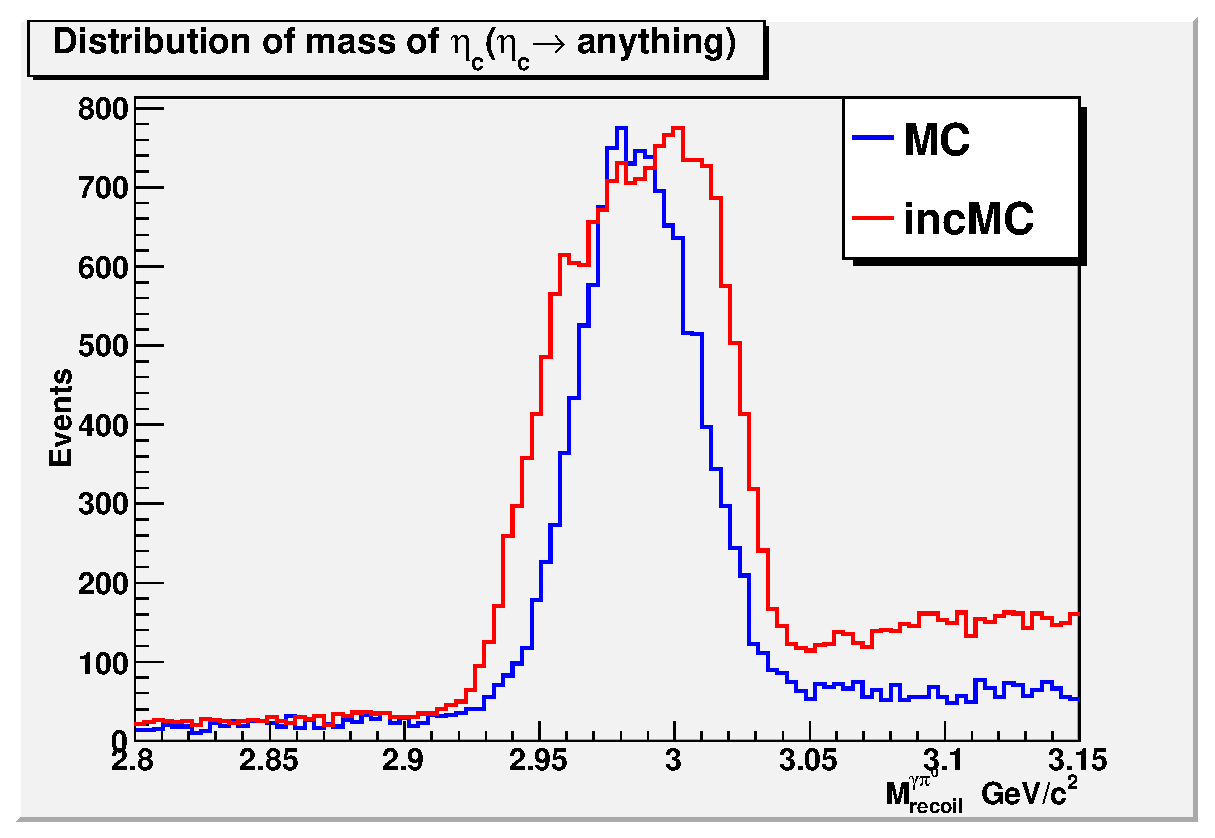
\includegraphics[width=1\textwidth,angle=0]{figures/Pi0hc_recoil_mass_of_etac.eps}\\
Mass distribution of $\eta_c$
\end{center}
\end{column}
\begin{column}{0.5\textwidth}
\begin{center}
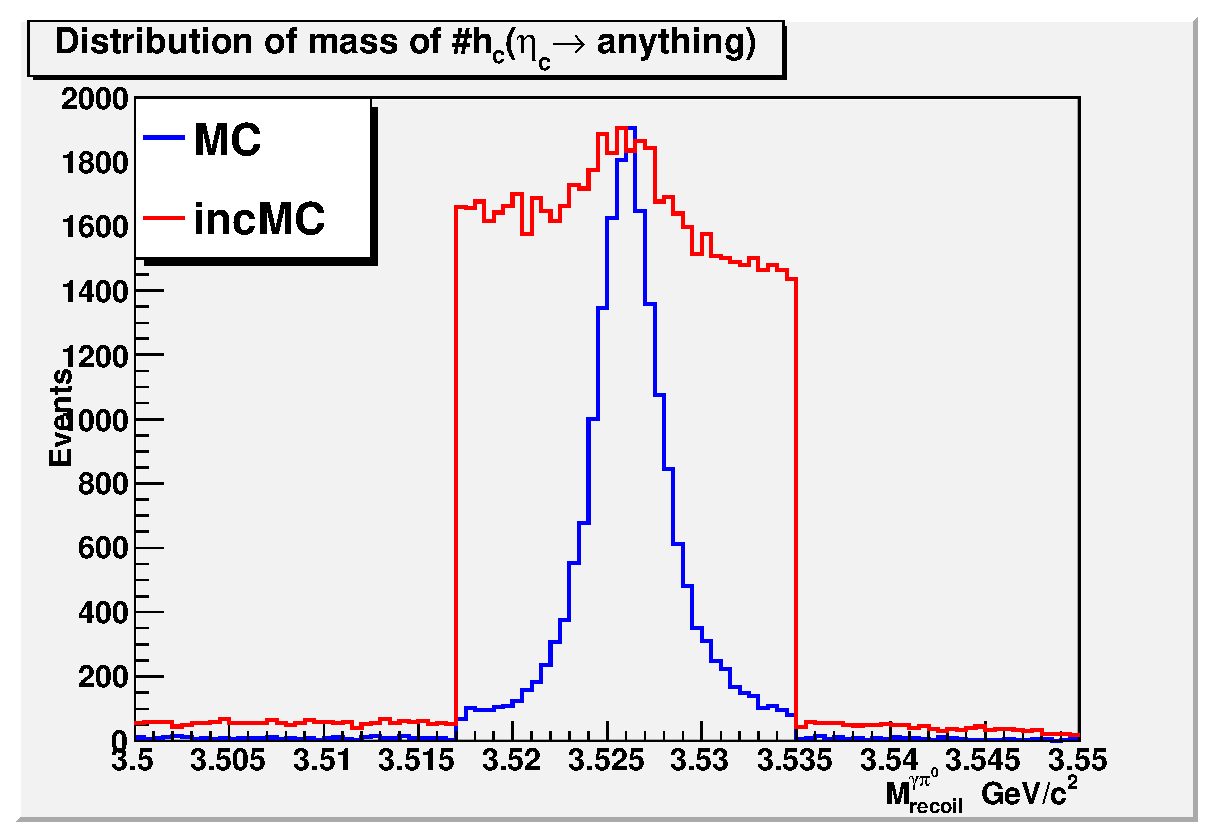
\includegraphics[width=0.8\textwidth,angle=0]{figures/Pi0hc_recoil_mass_of_hc.eps}\\
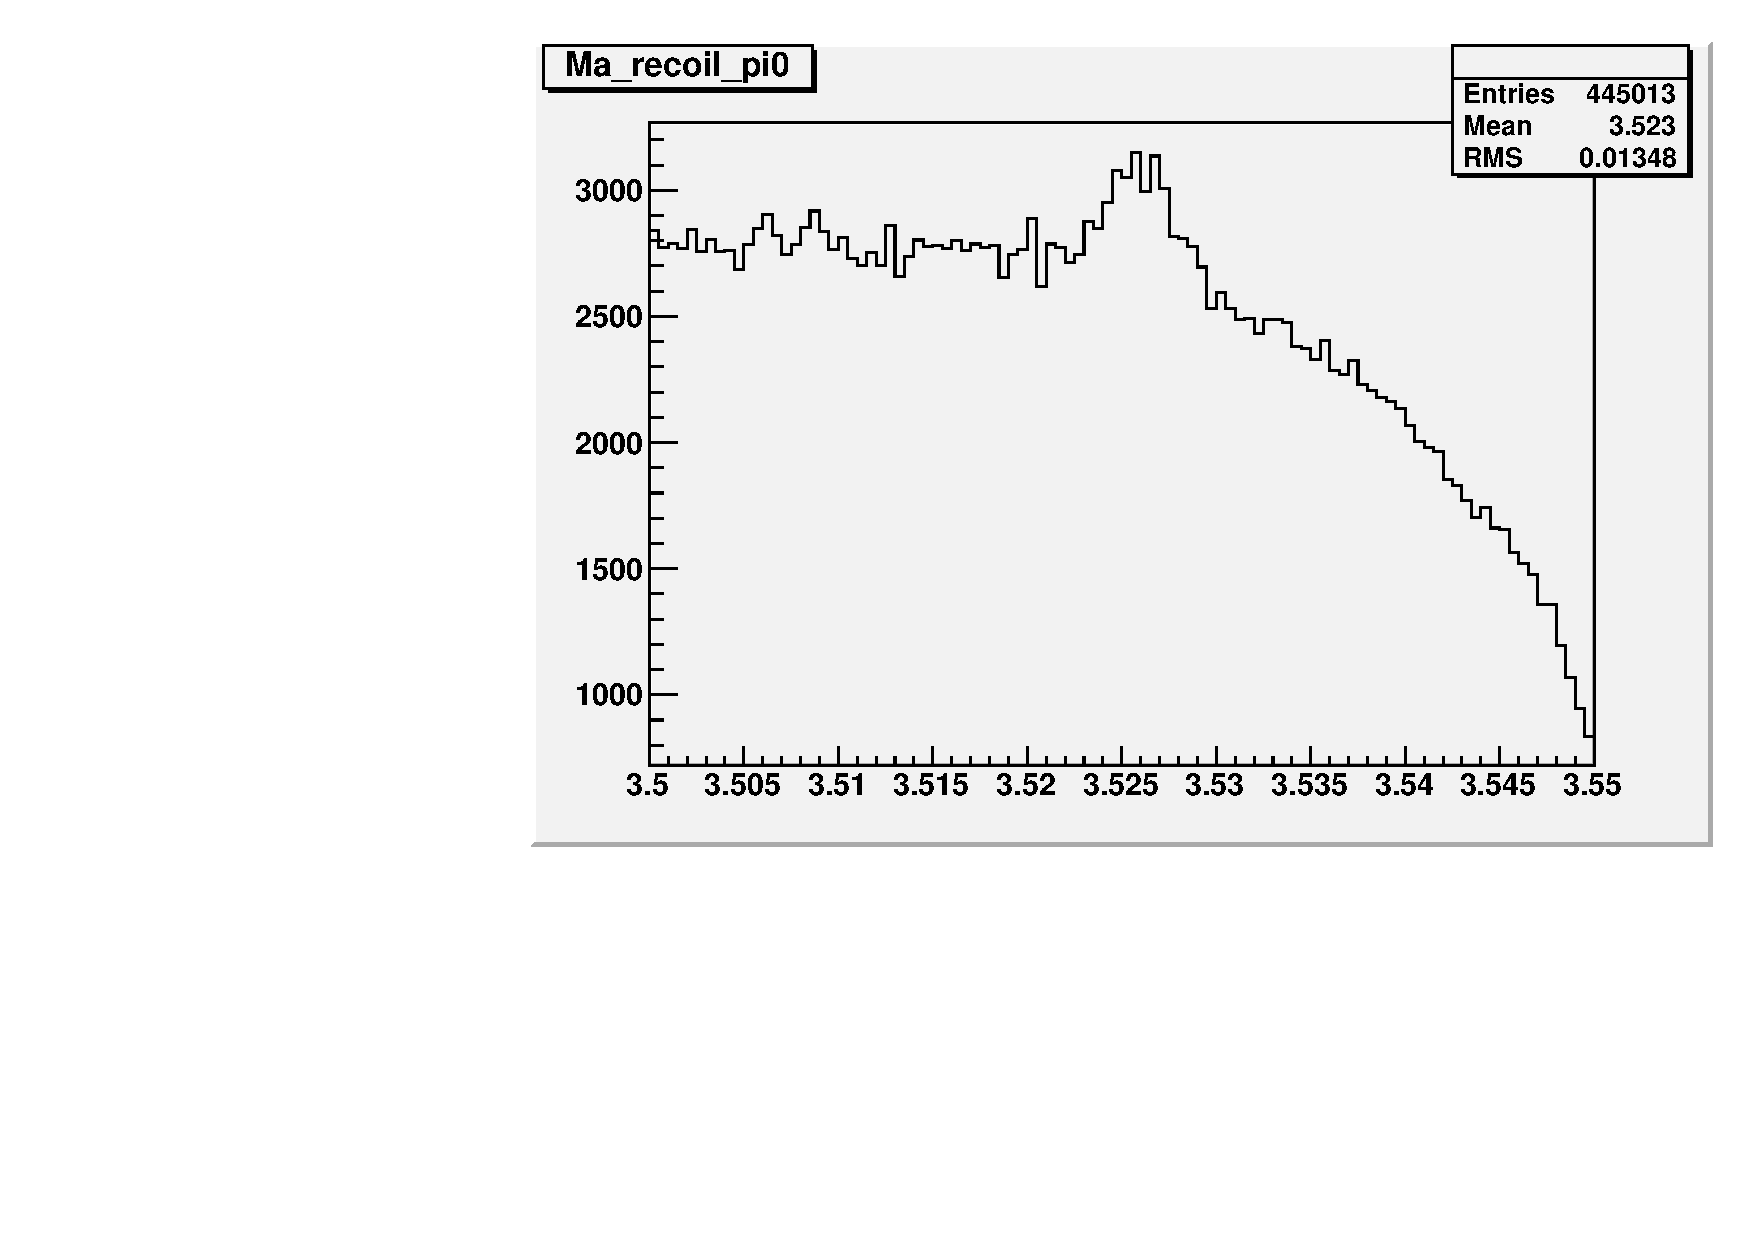
\includegraphics[width=0.4\textheight,angle=0]{figures/Pi0_recoil.pdf}\\
Mass distribution of $h_c$
\end{center}
\end{column}
\end{columns}
\end{frame}
%----------------------------------------------------------------------------------------
\begin{frame}{Topology analysis}
\vskip -1.5cm
\includegraphics[width=0.8\textwidth, angle=270]{figures/notice_recoil.eps}
\end{frame}
%----------------------------------------------------------------------------------------

\section{Work to be done}
\subsection{Work to be done}
%----------------------------------------------------------------------------------------
\begin{frame}{Work to do}
%\begin{block}
\begin{itemize}
\item Background study for the inclusive process
\item Fit the $\gamma$ $\pi^0$ recoil mass
\item Do IO check for inclusive process
\item Run data to get the branching ratio
\end{itemize}
%\end{block}
\end{frame}
%----------------------------------------------------------------------------------------
%----------------------------------------------------------------------------------------

\end{document}
%----------------------------------------------------------------------------------------
%----------------------------------------------------------------------------------------
